\documentclass[11pt]{article}
\usepackage[margin=1in]{geometry}
\usepackage{amsmath,amssymb,amsthm,graphicx,booktabs}
\usepackage{tikz,tikz-cd}
\usepackage{algorithm,algpseudocode}
\usepackage[inline]{enumitem}
\usepackage{changes}
\usepackage{hyperref}
\usetikzlibrary{arrows.meta,positioning}
% Macros live in their own file. The page reads them across \input.
\newcommand{\R}{\mathbb{R}}
\newcommand{\E}{\mathbb{E}}
\newcommand{\loss}{\mathcal{L}}
\newcommand{\norm}[1]{\left\lVert #1 \right\rVert}


\newtheorem{theorem}{Theorem}
\newtheorem{lemma}[theorem]{Lemma}
\theoremstyle{definition}
\newtheorem{definition}{Definition}

\title{Everything a Paper Can Do}
\author{Try Changing Anything Here}
\date{}

\begin{document}
\maketitle

\begin{abstract}
This file is for trying things. Click anywhere and type, press the play button at the top right
to build the PDF beside it, and click the PDF to come back to that place in the source.
\end{abstract}

\section{Introduction}\label{sec:intro}

Attention~\cite{vaswani17} is a weighted average, and typesetting~\cite{knuth84} is a craft. Text
can be \textbf{bold}, \emph{emphasised}, \underline{underlined} or \texttt{typewriter}, and a
footnote\footnote{Footnotes keep their place, and show on the page.} sits where it's cited.

Macros from \texttt{macros.tex} work on the page too: $\loss(\theta) \in \R$ and
$\norm{x}_2 \le \E[y]$. Click a formula to edit it, with the result in view.

\section{Method}\label{sec:method}

\subsection{Equations}

The objective is numbered in the margin, and references to it keep up:
\begin{equation}\label{eq:objective}
  \loss(\theta) = \E_{x \sim p}\bigl[\ell(f_\theta(x))\bigr] + \lambda \norm{\theta}_2^2 .
\end{equation}
Aligned steps each take a number, and limits stand under operators:
\begin{align}
  \theta_{t+1} &= \theta_t - \eta \nabla \loss(\theta_t) \label{eq:step} \\
  \hat\theta &= \operatorname*{arg\,min}_{\theta \in \R^d} \loss(\theta) \label{eq:best} \\
  \sum_{i=1}^{n} \alpha_i &= \prod_{j=1}^{m} 1 = \max_{k} 1 .
\end{align}
Equation~\eqref{eq:step} minimises~\eqref{eq:objective}. Matrices and cases work as well:
\[
  A = \begin{pmatrix} 1 & 0 \\ 0 & \lambda \end{pmatrix}, \quad
  \eta_t = \begin{cases} \eta_0 & t < T_0 \\ \eta_0 / \sqrt{t} & \text{otherwise.} \end{cases}
\]

\subsection{Theorems}

\begin{definition}[Weights]
The weights are $\alpha_{ij} = \exp(s_{ij}) / \sum_k \exp(s_{ik})$.
\end{definition}

\begin{theorem}[Main bound]\label{thm:main}
Let $\lambda > 0$. Then for every $T$,
\begin{equation}\label{eq:bound}
  R_T \le C \sqrt{T \log d}.
\end{equation}
\end{theorem}

\begin{lemma}\label{lem:sum}
The weights sum to one.
\end{lemma}

\begin{proof}
Immediate from the definition, which is why Theorem~\ref{thm:main} needs nothing more.
\end{proof}

\subsection{Lists}

\begin{itemize}
  \item A bullet, with $x^2$ in it.
  \item Another, with a list inside:
  \begin{enumerate}
    \item First.
    \item Second.
  \end{enumerate}
\end{itemize}

\subsection{Algorithms}

Anything the page can't draw itself is built alone by your LaTeX engine and appears when it's ready.

\begin{algorithm}[h]
\caption{Gradient descent}\label{alg:descent}
\begin{algorithmic}[1]
\Require step size $\eta > 0$
\For{$t = 1, \dots, T$}
  \State $\theta_{t+1} \gets \theta_t - \eta g_t$
\EndFor
\end{algorithmic}
\end{algorithm}

\subsection{Diagrams}

A commutative square, drawn from its source:

\begin{tikzcd}
  A \arrow[r, "f"] \arrow[d, "g"'] & B \arrow[d, "h"] \\
  C \arrow[r, "k"'] & D
\end{tikzcd}

And a figure in TikZ, with its caption and number:

\begin{figure}[h]
\centering
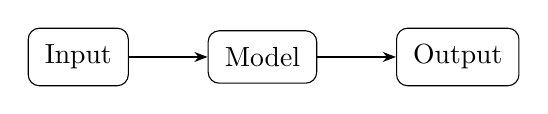
\begin{tikzpicture}[>=Stealth, every node/.style={draw, rounded corners, inner sep=6pt}]
  \node (a) {Input};
  \node[right=of a] (b) {Model};
  \node[right=of b] (c) {Output};
  \draw[->] (a) -- (b);
  \draw[->] (b) -- (c);
\end{tikzpicture}
\caption{The pipeline.}\label{fig:pipeline}
\end{figure}

\section{Results}\label{sec:results}

This section lives in its own file, and its numbering carries on from the main one, as
Table~\ref{tab:results} and Figure~\ref{fig:loss} show. Right-click a table cell for rows and columns.

\begin{table}[h]
  \centering
  \begin{tabular}{lrr}
    \hline
    Model & Accuracy & Params \\
    \hline
    Baseline & 91.2 & 1.2M \\
    Attention & 94.8 & 1.4M \\
    \hline
  \end{tabular}
  \caption{Accuracy on the test set.}\label{tab:results}
\end{table}

\begin{figure}[h]
  \centering
  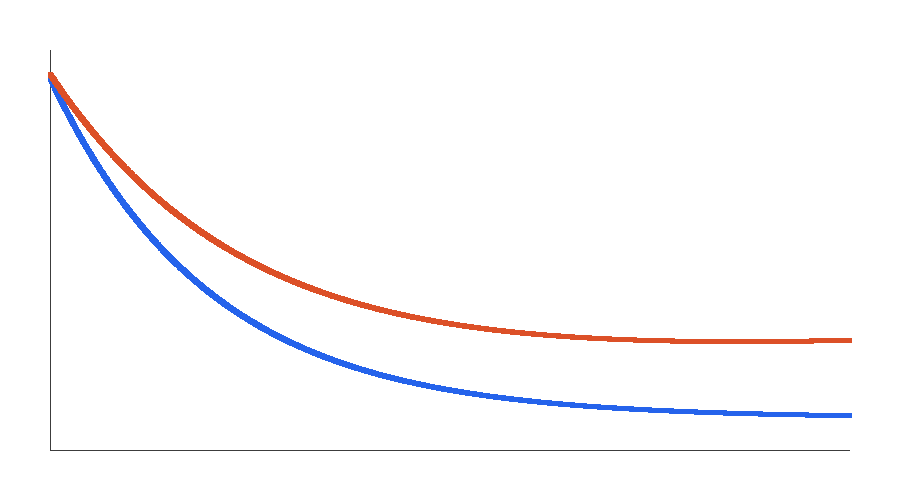
\includegraphics[width=0.7\linewidth]{figures/loss}
  \caption{Training and validation loss.}\label{fig:loss}
\end{figure}


\section{Track changes}\label{sec:changes}

The pencil in the bar keeps your edits as suggestions, and a right click settles them. This
sentence \added{gains these words}, \deleted{loses these}, and \replaced{has a new word}{has an old word}.

\section{Spelling}

This sentance has a mispelled word on purpose. Right-click it for fixes.

\appendix

\section{Proofs}\label{app:proofs}

The numbering of a section changes here, as it does in print.

\bibliographystyle{plain}
\bibliography{refs}

\end{document}
